\documentclass{article}

\usepackage[utf8]{inputenc}
\usepackage[english]{babel}

\usepackage{amsmath,amsfonts,amssymb}
\usepackage{fullpage}
\usepackage{verbatim}
\usepackage{mathabx}

\usepackage{tikz,pgfplots}

\pgfplotsset{
  width=150mm,height=100mm,
  major grid style={thin,dotted,color=black!50},
  minor grid style={thin,dotted,color=black!50},
  grid,
  every axis/.append style={
    line width=0.5pt,
    tick style={
      line cap=round,
      thin,
      major tick length=4pt,
      minor tick length=2pt,
    },
  },
  legend cell align=left,
  legend pos=north west,
}

%%%%%%%%%%%%%%%%%%%%%%%%%%%%%%%%%%%%%%%%%%%%%%%%%%%%%%%%%%%%%%%%%%%%%%%%%%%%%%%%

\begin{document}

\title{LCE-Queries}
\author{Alexander Herlez}
%\maketitle



% IMPORT-DATA stats time-2019-10-30-21-25-05.txt

\begin{center}
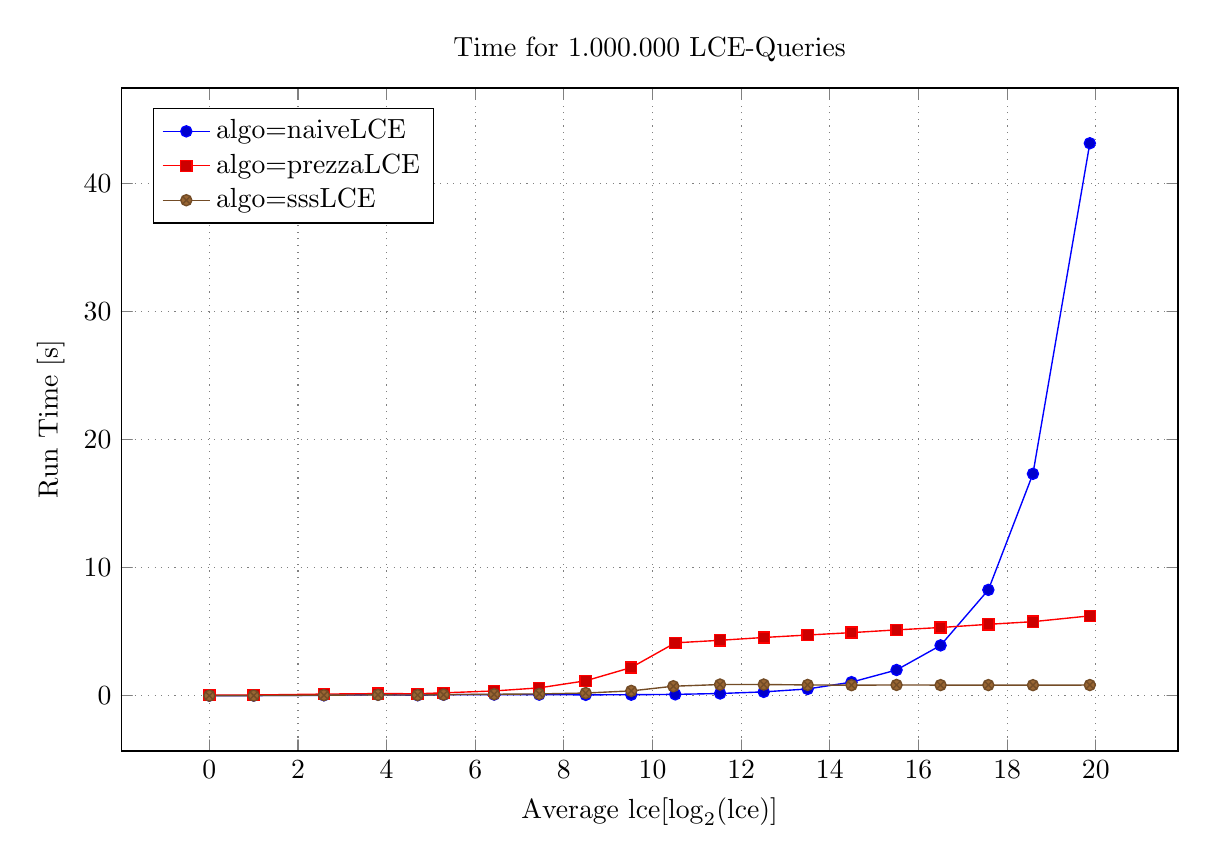
\begin{tikzpicture}
  \begin{axis}[
    title={Time for 1.000.000 LCE-Queries},
    xlabel={Average lce[$\log_2$(lce)]},
    ylabel={Run Time [s]},
    ]

    %% MULTIPLOT(algo) SELECT LOG(2, aveLCE) AS x, time AS y, MULTIPLOT
    %% FROM stats GROUP BY MULTIPLOT,x  ORDER BY MULTIPLOT,x
    \addplot coordinates { (0.0,0.00274205) (1.0,0.0065949) (2.58496,0.0309031) (3.80735,0.0779071) (4.70044,0.0358331) (5.2854,0.0747321) (6.42626,0.0853648) (7.44294,0.0812061) (8.49185,0.0637929) (9.51964,0.075532) (10.5127,0.10263) (11.5241,0.170322) (12.5085,0.297081) (13.4995,0.52491) (14.4891,1.05922) (15.505,2.00928) (16.4984,3.93021) (17.5768,8.26997) (18.5825,17.3422) (19.8661,43.1784) };
    \addlegendentry{algo=naiveLCE};
    \addplot coordinates { (0.0,0.046844) (1.0,0.051378) (2.58496,0.125169) (3.80735,0.163161) (4.70044,0.151209) (5.2854,0.223049) (6.42626,0.369886) (7.44294,0.610668) (8.49185,1.16453) (9.51964,2.20206) (10.5127,4.13067) (11.5241,4.32946) (12.5085,4.54928) (13.4995,4.74085) (14.4891,4.92845) (15.505,5.14243) (16.4984,5.32838) (17.5768,5.57708) (18.5825,5.78447) (19.8661,6.23809) };
    \addlegendentry{algo=prezzaLCE};
    \addplot coordinates { (0.0,0.00383687) (1.0,0.00745106) (2.58496,0.038883) (3.80735,0.063612) (4.70044,0.04774) (5.2854,0.079807) (6.42626,0.111833) (7.44294,0.136136) (8.49185,0.206968) (9.51964,0.37483) (10.4686,0.738834) (11.5216,0.871517) (12.5085,0.873005) (13.4995,0.839543) (14.4891,0.819609) (15.505,0.839114) (16.4984,0.827524) (17.5768,0.829085) (18.5825,0.823539) (19.8661,0.831587) };
    \addlegendentry{algo=sssLCE};

  \end{axis}
\end{tikzpicture}
\end{center}

\end{document}
